\documentclass[11pt,a4paper]{article}

\newcommand{\ROOT}[0]{/Users/atlytle/Dropbox/Tex_docs}
\usepackage{\ROOT/jheppub}
\usepackage{\ROOT/mystyle}
\graphicspath{{./figs/}}

\title{\boldmath $\Delta_\text{mix}$ for overlap on a HISQ sea.}
\author{S.\ Basak,}
\author{A.T.\ Lytle,}
\author{N. Mathur,}
\author{...}
\abstract{...}

\begin{document}
\maketitle
\section{Research}
We have in mind something along the lines of~\cite{Lujan:2012wg} which looks at overlap
on domain-wall.  The ``master formula'' involves pseudoscalar meson masses determined
using propagators calculated from both valence and sea Dirac operators.
A similar approach is used in~\cite{Aubin:2008wk} for domain-wall on asqtad.
The determination of $a^2 \Delta_\text{mix}$ extends the work of~\cite{Orginos:2007tw} to the fine asqtad ensemble.
The prior work computed on only the coarse and uses yet another parametrization which 
appears well-justified based on that paper's discussion.
For overlap on HISQ the pseudoscalar
masses at LO are given as:
\begin{align}
m^2_{vv'} &= B_{\text{ov}} (m_v + m_{v'}) \\
m^2_{ss'} &= B_{\text{HISQ}}(m_s + m_{s'}) + a^2 \Delta_{t} \label{ss'}\\
m^2_{vs} &= B_{\text{ov}} m_v + B_{\text{HISQ}} m_s + a^2 \Delta_\text{mix} \label{vs}
\end{align}
$\Delta_t$ measures taste-breaking and in particular vanishes for the taste-5 GB pion.
I am unclear on whether there is an additional $\Delta_{\text{sea}}$ term
arising in~\eqref{ss'} and~\eqref{vs} when the valence sea-mass doesn't match the sea mass,
but it looks like there is not such a term.. I need to understand this better.
Some theory references:~\cite{Aubin:2003mg}\cite{Bar:2005tu}\cite{Chen:2006wf}

Ref.~\cite{Orginos:2007tw} has details of constructing the ``Wilsonized" propagator
from the staggered propagator, i.\ e.\ a 4-component object,
and also many useful details regarding the fit-forms of the two-pt functions.  I think is just the inverse
of the Wilson $\rightarrow$ staggered transformation, and it is implemented in {\tt inline\_stag\_to\_wils.cc} in Chroma.

\subsection{Overlap on HISQ propagators - Measurement Strategy}
I am successfully parsing the overlap propagators, with results for pion correlators that agree
with Nilmani for both single and double mass propagators.  We need to discuss what all data is available and where (including what I may have already), and how much of that we want to run the measurements on..
\subsection{HISQ propagators}
Right now we are looking at the $24^3 \times 64$ HISQ ensembles with dynamical charm~\cite{Bazavov:2012xda}.
We have unitary propagators for the following masses (cf  Table IX p.16):
\begin{verbatim}
6.00(24^3X64) : 0.0102(m_l) 0.0509(m_s) 0.635(m_c)
6.30(32^3X96) : 0.0074 (m_l) 0.037(m_s) 0.440
6.72(48^3X144) : 0.0048 (m_l) 0.024(m_s) 0.286
\end{verbatim}
On $24^3 \times 64$ there are 81 configurations.

I find that the ``kaon'' effective mass plots have an oscillatory behavior, as compared to 
the pions.  
%For example see Fig.[].  
I would like to understand this better.
In practice I still fit the standard cosh form because I think the oscillating state has a much higher mass. Preliminary results for all combination of HISQ masses are in Fig.~\ref{HH_pseudo}.% and [].
\begin{figure}[h]
\centering
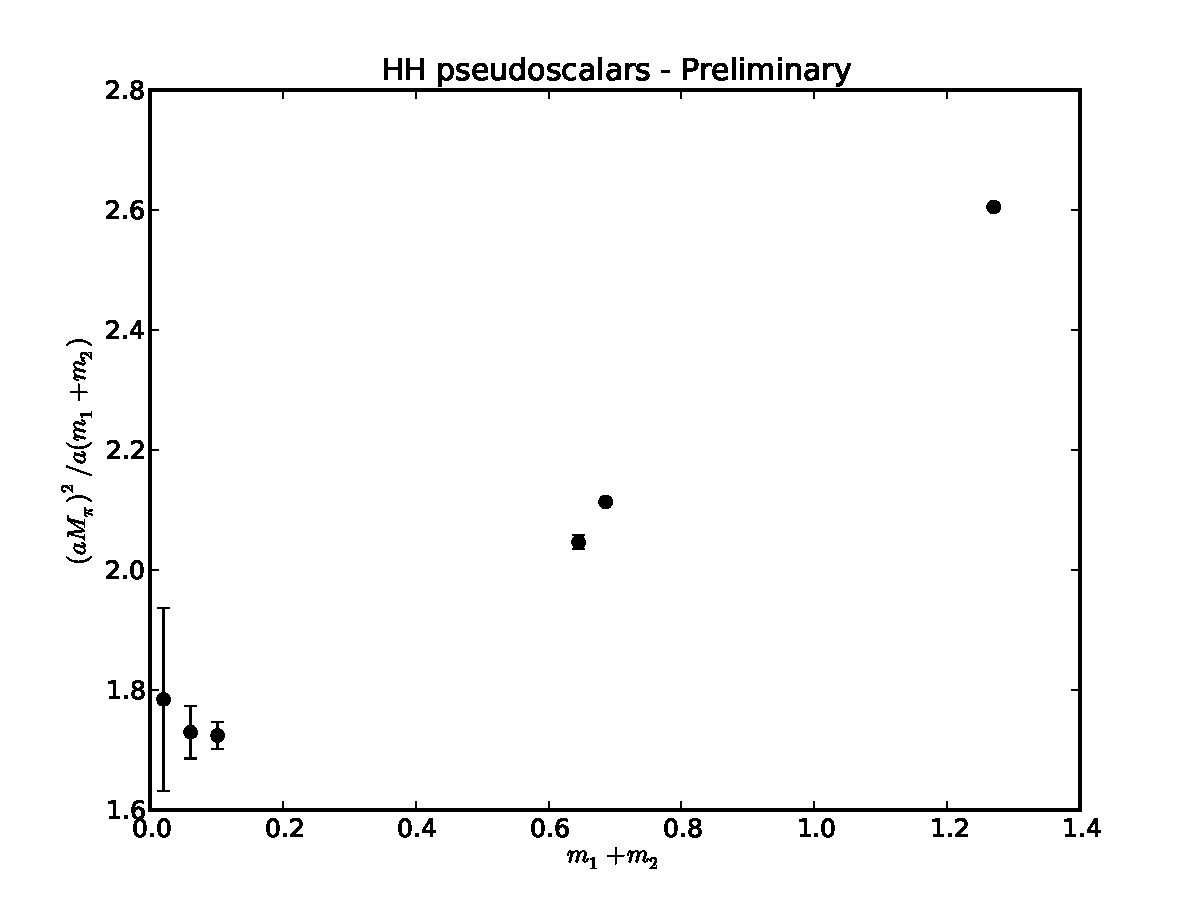
\includegraphics[width=\textwidth]{HH_pseudo}
\caption{HISQ valence on HISQ sea.  We see flat behavior in the pion-kaon mass range, whereas
when including the charm mass clearly~\ref{ss'} breaks down.}
\label{HH_pseudo}
\end{figure}

HISQ propagators are constructed using a ``corner wall" source.  This source is 1 at all sites
$\{ (\mathbf{x}, t) \, | \, \mathbf{x} \% 2 = \mathbf{0} \text{ and } t = t_0\}$.

%-------------------Bibliography-------------------

\bibliographystyle{JHEP}
\bibliography{\ROOT/myrefs}

\end{document}  